\documentclass[a4paper, 11pt]{article}
\usepackage{amsmath}
\usepackage[utf8]{inputenc}
\usepackage{lmodern}
\usepackage[T1]{fontenc}
\usepackage{textcomp}
\usepackage{comment}
\usepackage{fullpage} % changes the margin
\usepackage{graphicx}
\graphicspath{ {data/images/} }

\begin{document}

\section*{CoGaDB}
\section*{Overview}
CoGaDB\footnote{http://cogadb.dfki.de/} is a column-oriented coprocessor-accelerated database system which effectively provides a high performance OLAP engine that makes efficient use of GPUs, CPUs or MICs (Xeon Phi) for query processing. This system is developed by the DIMA\footnote{https://www.dima.tu\text{-}berlin.de/menue/database\_systems\_and\_information\_management\_group/} group at Berlin and the IAM\footnote{https://www.dfki.de/web/forschung/iam/} group at German Research Center for Artificial Intelligence.
\\
CoGaDB implements a specialized cost modelling algorithm for selection of the most efficient heterogeneous processor environment using parallel query processor and \emph{Hybrid Query Processing Engine}(HyPE)\cite{cogadb_hype}. It also uses a customized query compiler called Hawk\cite{cogadb_hawk} for generation of specialized code for different processors which is highly optimized depending upon the query workload and data set.

\subsubsection*{HyPE - Hybrid Query Processing Engine}
HyPE is hybrid query processing engine that helps in selecting the best possible processing system from the pool of heterogeneous processing units based on effective cost models and query plans. It is driven on the decision modelling algorithms and perform the following tasks\cite{cogadb_hype}: (1) estimation of operators cost with respect to data locality, (2) strategies for hybrid query optimizations, and (3) selecting the most optimized query plan.

\subsection*{Hawk - Hardware Adaptive Query Compiler}
The processor vendors need to specialize their hardware depending on the application specification due to energy budget and power wall\cite{microprocessors} constraint. Due to this, several heterogeneous processors are implemented which increases the hardware complexity for any database system. This purpose of Hawk\cite{cogadb_hawk} is to solve this complexity by adapting query compilers and interpreters depending upon the hardware specification. It introduces variations in database operations depending upon the processing unit due to which it is an extremely critical component for CoGaDB's coprocessor-accelerated implementation.

\section*{Architecture}
S Bre{ß} and others developed CoGaDB architecture to be highly efficient and modularized as shown in top-down approach in Figure \ref{fig:cogadbarch}.
As most DBMSs, CoGaDB provides SQL frontend interface which can be used to write SQL language queries and launch it to get results from database. The SQL interface converts the provided language query into abstract syntax tree which is then pushed to logical optimizer module after being converted into a logical plan. Then, CoGaDB's logical optimizer applies pre-defined optimization policies on the logical plan such as pushing down selections, cross products resolution and reviewing join conditions. After this, the more efficient logical query plan is provided to HyPE for processing.
\begin{figure}
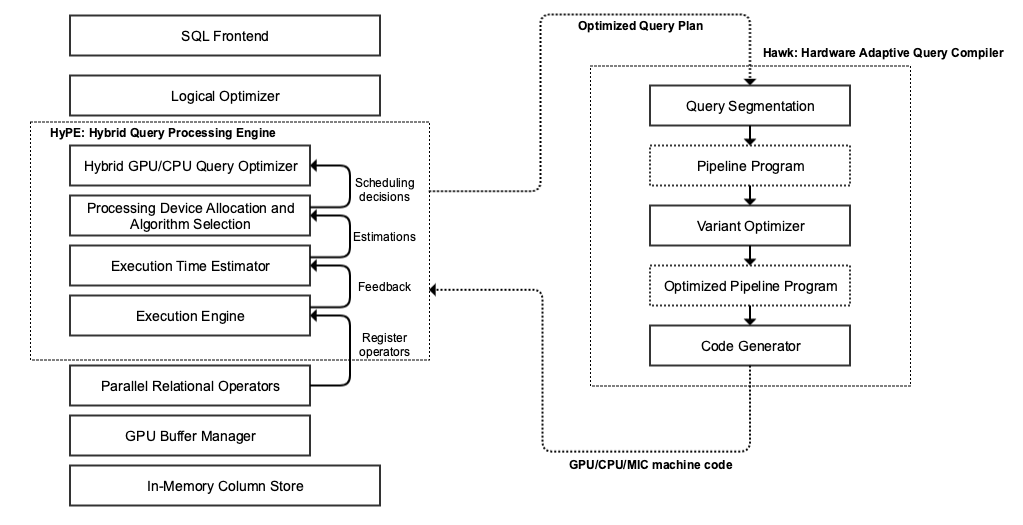
\includegraphics[width=\textwidth]{cogadb_hawk_architecture}
\caption{The architecture of CoGaDB, adapted from \cite{cogadb_hawk} and \cite{cogadb_manual}}
\label{fig:cogadbarch}
\end{figure}


\section*{Exploring the design-space}
\subsection*{Non-functional properties}
\subsubsection*{Performance}
Performance

\subsubsection*{Portability}
Portability

\subsection*{Functional properties}
\subsubsection*{Storage system}
Storage System

\subsubsection*{Storage model}
Storage model

\subsubsection*{Processing model}
Processing Model

\subsubsection*{Buffer management}
Buffer management

\subsubsection*{Query Placement and Optimisation}
Query Placement and Optimisation

\subsubsection*{Consistency and Transaction Processing}
Consistency and Transaction Processing


\begin{thebibliography}{9}
\bibitem{cogadb_design_impl} 
Sebastian Bre{ß}. The Design and Implementation of CoGaDB: A Column-oriented GPU-accelerated DBMS. \emph{Datenbank Spektrum}, $14:199\text{-}209,2014$ 
\bibitem{cogadb_hype}  S. Breß. Why it is time for a HyPE: A hybrid query processing engine for efficient
GPU coprocessing in dbms. \emph{The VLDB PhD workshop, PVLDB}, 6(12):1398–1403,2013
\bibitem{operator_gpu} S. Breß, N. Siegmund, L. Bellatreche, and G. Saake. An operator-stream-based
scheduling engine for effective GPU coprocessing. In \emph{ADBIS}, pages 288–301. Springer, 2013.
\bibitem{cogadb_hawk} S Breß, B Kocher, H Funke, S Zeuch, T Rabl and V Markl. Generating Custom Code for Efficient Query Execution on Heterogeneous Processors
\bibitem{microprocessors}S. Borkar and A. A. Chien. The future of microprocessors. \emph{Communications of the
ACM}, 54(5):67\text{–}77, 2011.
\bibitem{cogadb_manual}S. Breß, R. Haberkorn, and S. Ladewig. CoGaDB reference manual, 2014. \textbf{http://wwwiti.cs.uni-magdeburg.de/iti\_db/research/gpu/cogadb/0.3/doc/refman.pdf.}
\end{thebibliography}

\end{document}
